\chapter{Aufbau}

\section{Erste Planung}
Bei den anfänglichen Überlegungen stand schnell fest, dass wir uns auf zukunftsorientierte und bewährte Technologien
stützen wollen. Nach wenigen Stunden hatten wir dann schon eine Idee wie das
UML-Diagramm auszusehen hat. Nach diesem UML-Diagramm wurde dann die erste Datenbankstruktur erstellt.

\section{Komponenten}
Unser Projekt besteht aus insgesamt drei Komponenten, die miteinander kommunizieren.

\begin{itemize}
  \item \textbf{Server}: Der Server verwaltet die Daten des Projektes. Mithilfe von \textbf{HTTP}
        Anfragen können Daten modifiziert, verwaltet, gelöscht oder hinzugefügt werden.

  \item \textbf{Website}: Die Idee hinter der Webseite ist es, einen schnellen Überblick zu
        erschaffen. Skater sollen schnell Skateparks finden können und auch ihre Meinung zu den
        jeweiligen Parks teilen können. Außerdem sollten sie in der Lage sein einen Vorschlag von einem
        Park an die Seitenbetreiber zu schicken, welchen diesen dann in die Datenbank hinzufügen können.
        Die Administration der Anwendung erfolgt ebenfalls über die Seite.

  \item \textbf{Mobile}: Auch in der Handy-App ist es möglich sich alle Skateparks und ihre
        Position anzeigen zu lassen. Außerdem kann man die Parks nach der aktuellen Distanz sortieren,
        um sofort zu sehen welcher Skatepark am nächsten ist.
\end{itemize}

\begin{figure}[H]
  \begin{center}
    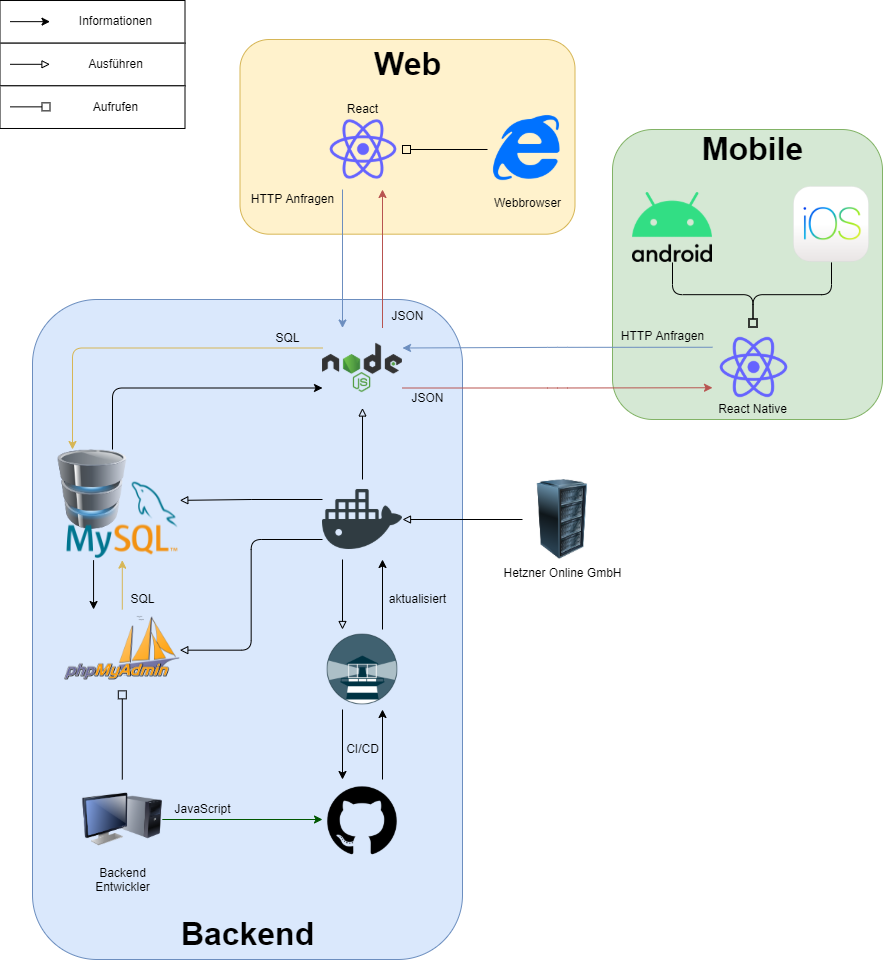
\includegraphics[width=0.85\textwidth]{Intro/Aufbau.png}
    \caption{Aufbau und Kommunikationswege des Projekts}
  \end{center}
\end{figure}

\paragraph{Web/Mobile}
Die Website und React Native App kommunizieren über HTTP-Anfragen mit der API, welche anschließend
die Daten im JSON-Format zurücksendet. Zum Beispiel werden über die Route "api/skateparks" alle
Parks mit Bildern von der Datenbank an den jeweiligen Client weitergeleitet.

\paragraph{Backend}
Der Backend-Entwickler pusht den fertigen JavaScript-Code auf das Github-Repository.
Der Watchtower der in einem eignen Docker-Container läuft bemerkt eine Änderung am Repository, darauf hin
pulled er den neusten Stand, erzeugt einen neuen Docker-Container und startet ihn. In diesem
Docker-Container liegt nun der NodeJs-Server. Diesen Vorgang nennt man \textbf{CI/CD}. \textit{PhpMyAdmin} ist das
Admin-Panel für die Datenbank. Jeder von uns hat darauf vollen Zugriff.